User Interface Design is an important aspect during the developing process of a system. It has the aim to model the part of the system that is related with users, hence it must be simple and efficient, in terms of accomplishing users' goals. Since user's schedule is the crucial point in \projectname~, we thought to use the calendar page as home page of the application in order to facilitate the actions that the user should do more often. Additionally UI of \projectname~ should be concise, responsive, professional and good-looking for the purpose of satisfying all the possible type of users that could interact with the system.\\
\\
In our charts, classes marked with * are the ones that will be analysed more accurately in other diagrams.\\
We are going to present 4 different UX diagrams:
\begin{itemize}
	\item{\textbf{Registration/Login}}: UX diagram of login and registration phase that can be done using external login providers. During the registration process users have to complete an input form inserting default locations, preference list and nickname. This is a crucial phase in order to use all system functionalities.
	\item{\textbf{Calendar Page}}: UX diagram of the home page seen by a user that shows the main actions available.
	\item{\textbf{Settings}}: UX diagram of the settings page of the system. It shows all the customizable feature such as preference list, default location, constraints, status and breaks.
	\item{\textbf{Notification}}: UX diagram that shows how notifications are managed by the system and how they can be used by users.
	\item{\textbf{Manage Meeting}}: UX diagram that shows all the screens and the available actions about meetings.
\end{itemize}

\begin{figure}[h]
	\centering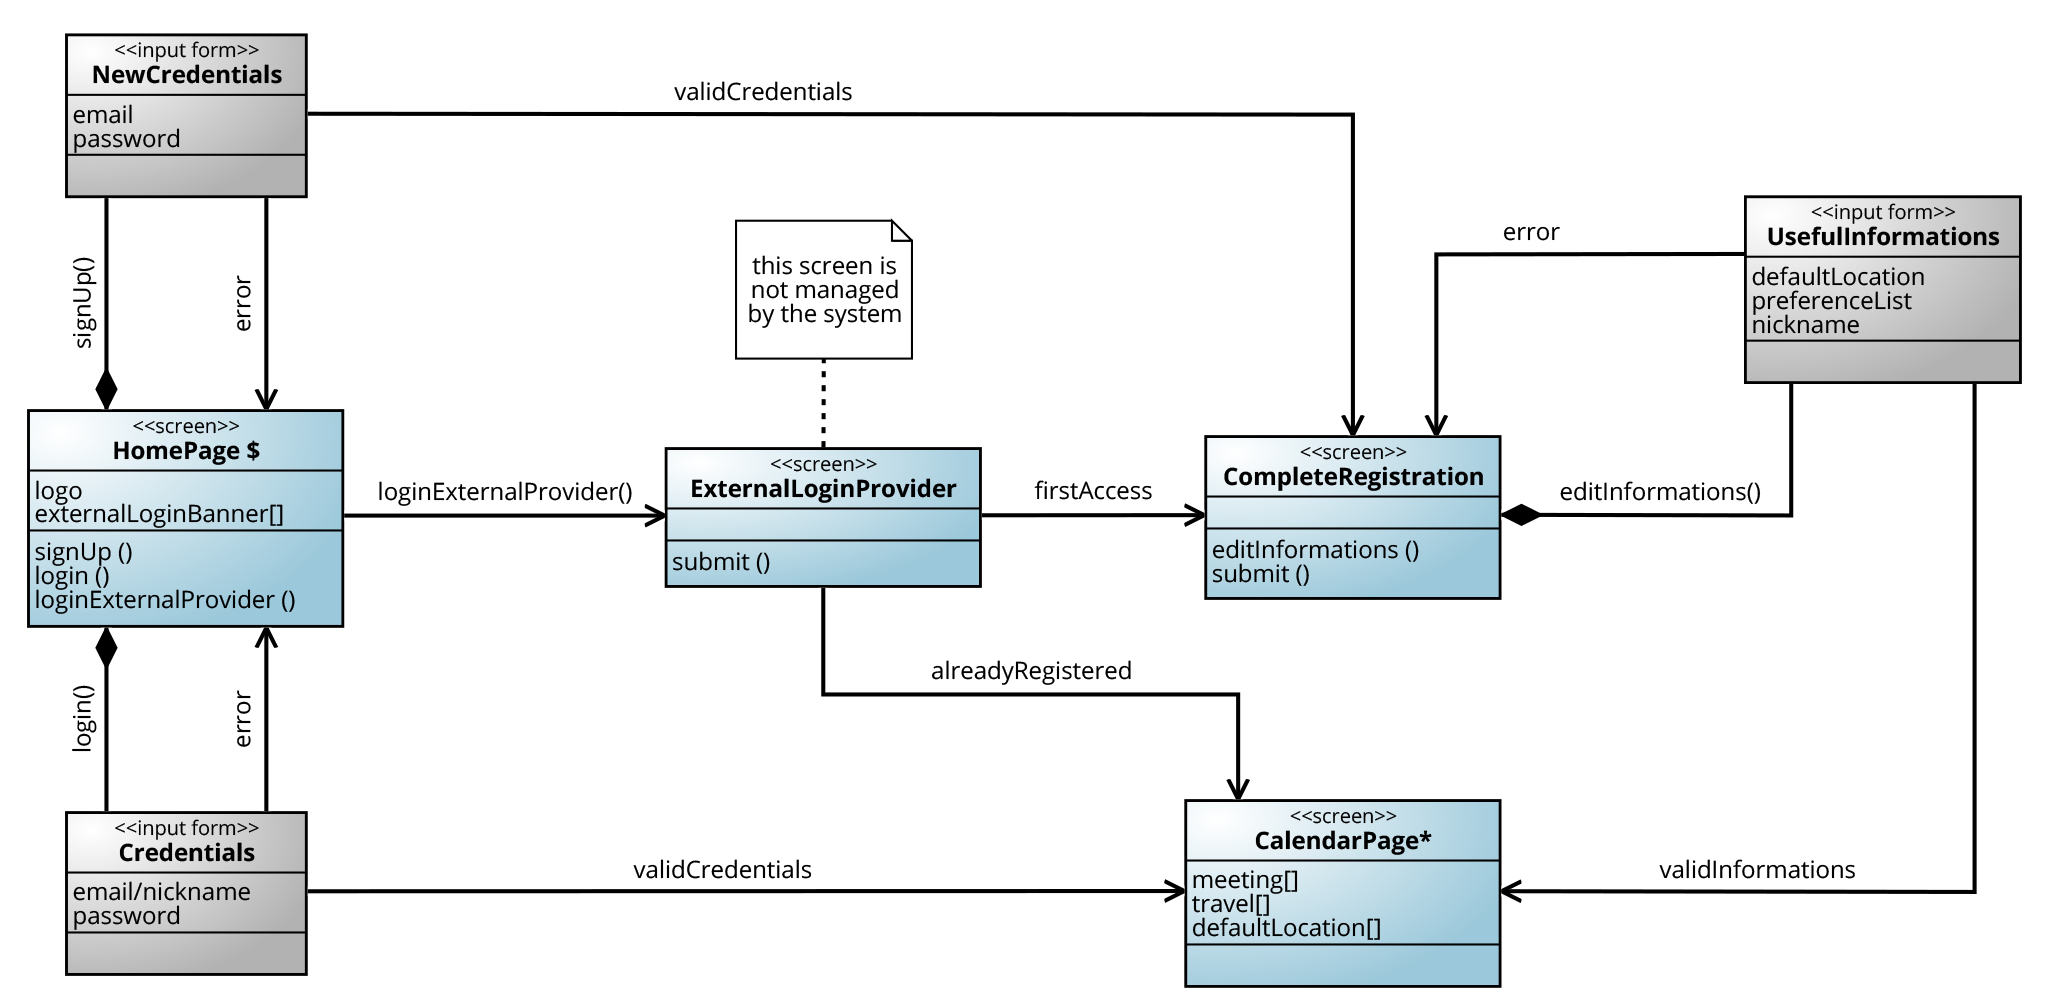
\includegraphics[ width=\textwidth, scale = 1]{Images/UX/UXRegistrationLogin.png}{}
	\caption{Registration and Login UX}
\end{figure}

\begin{figure}[h]
	\centering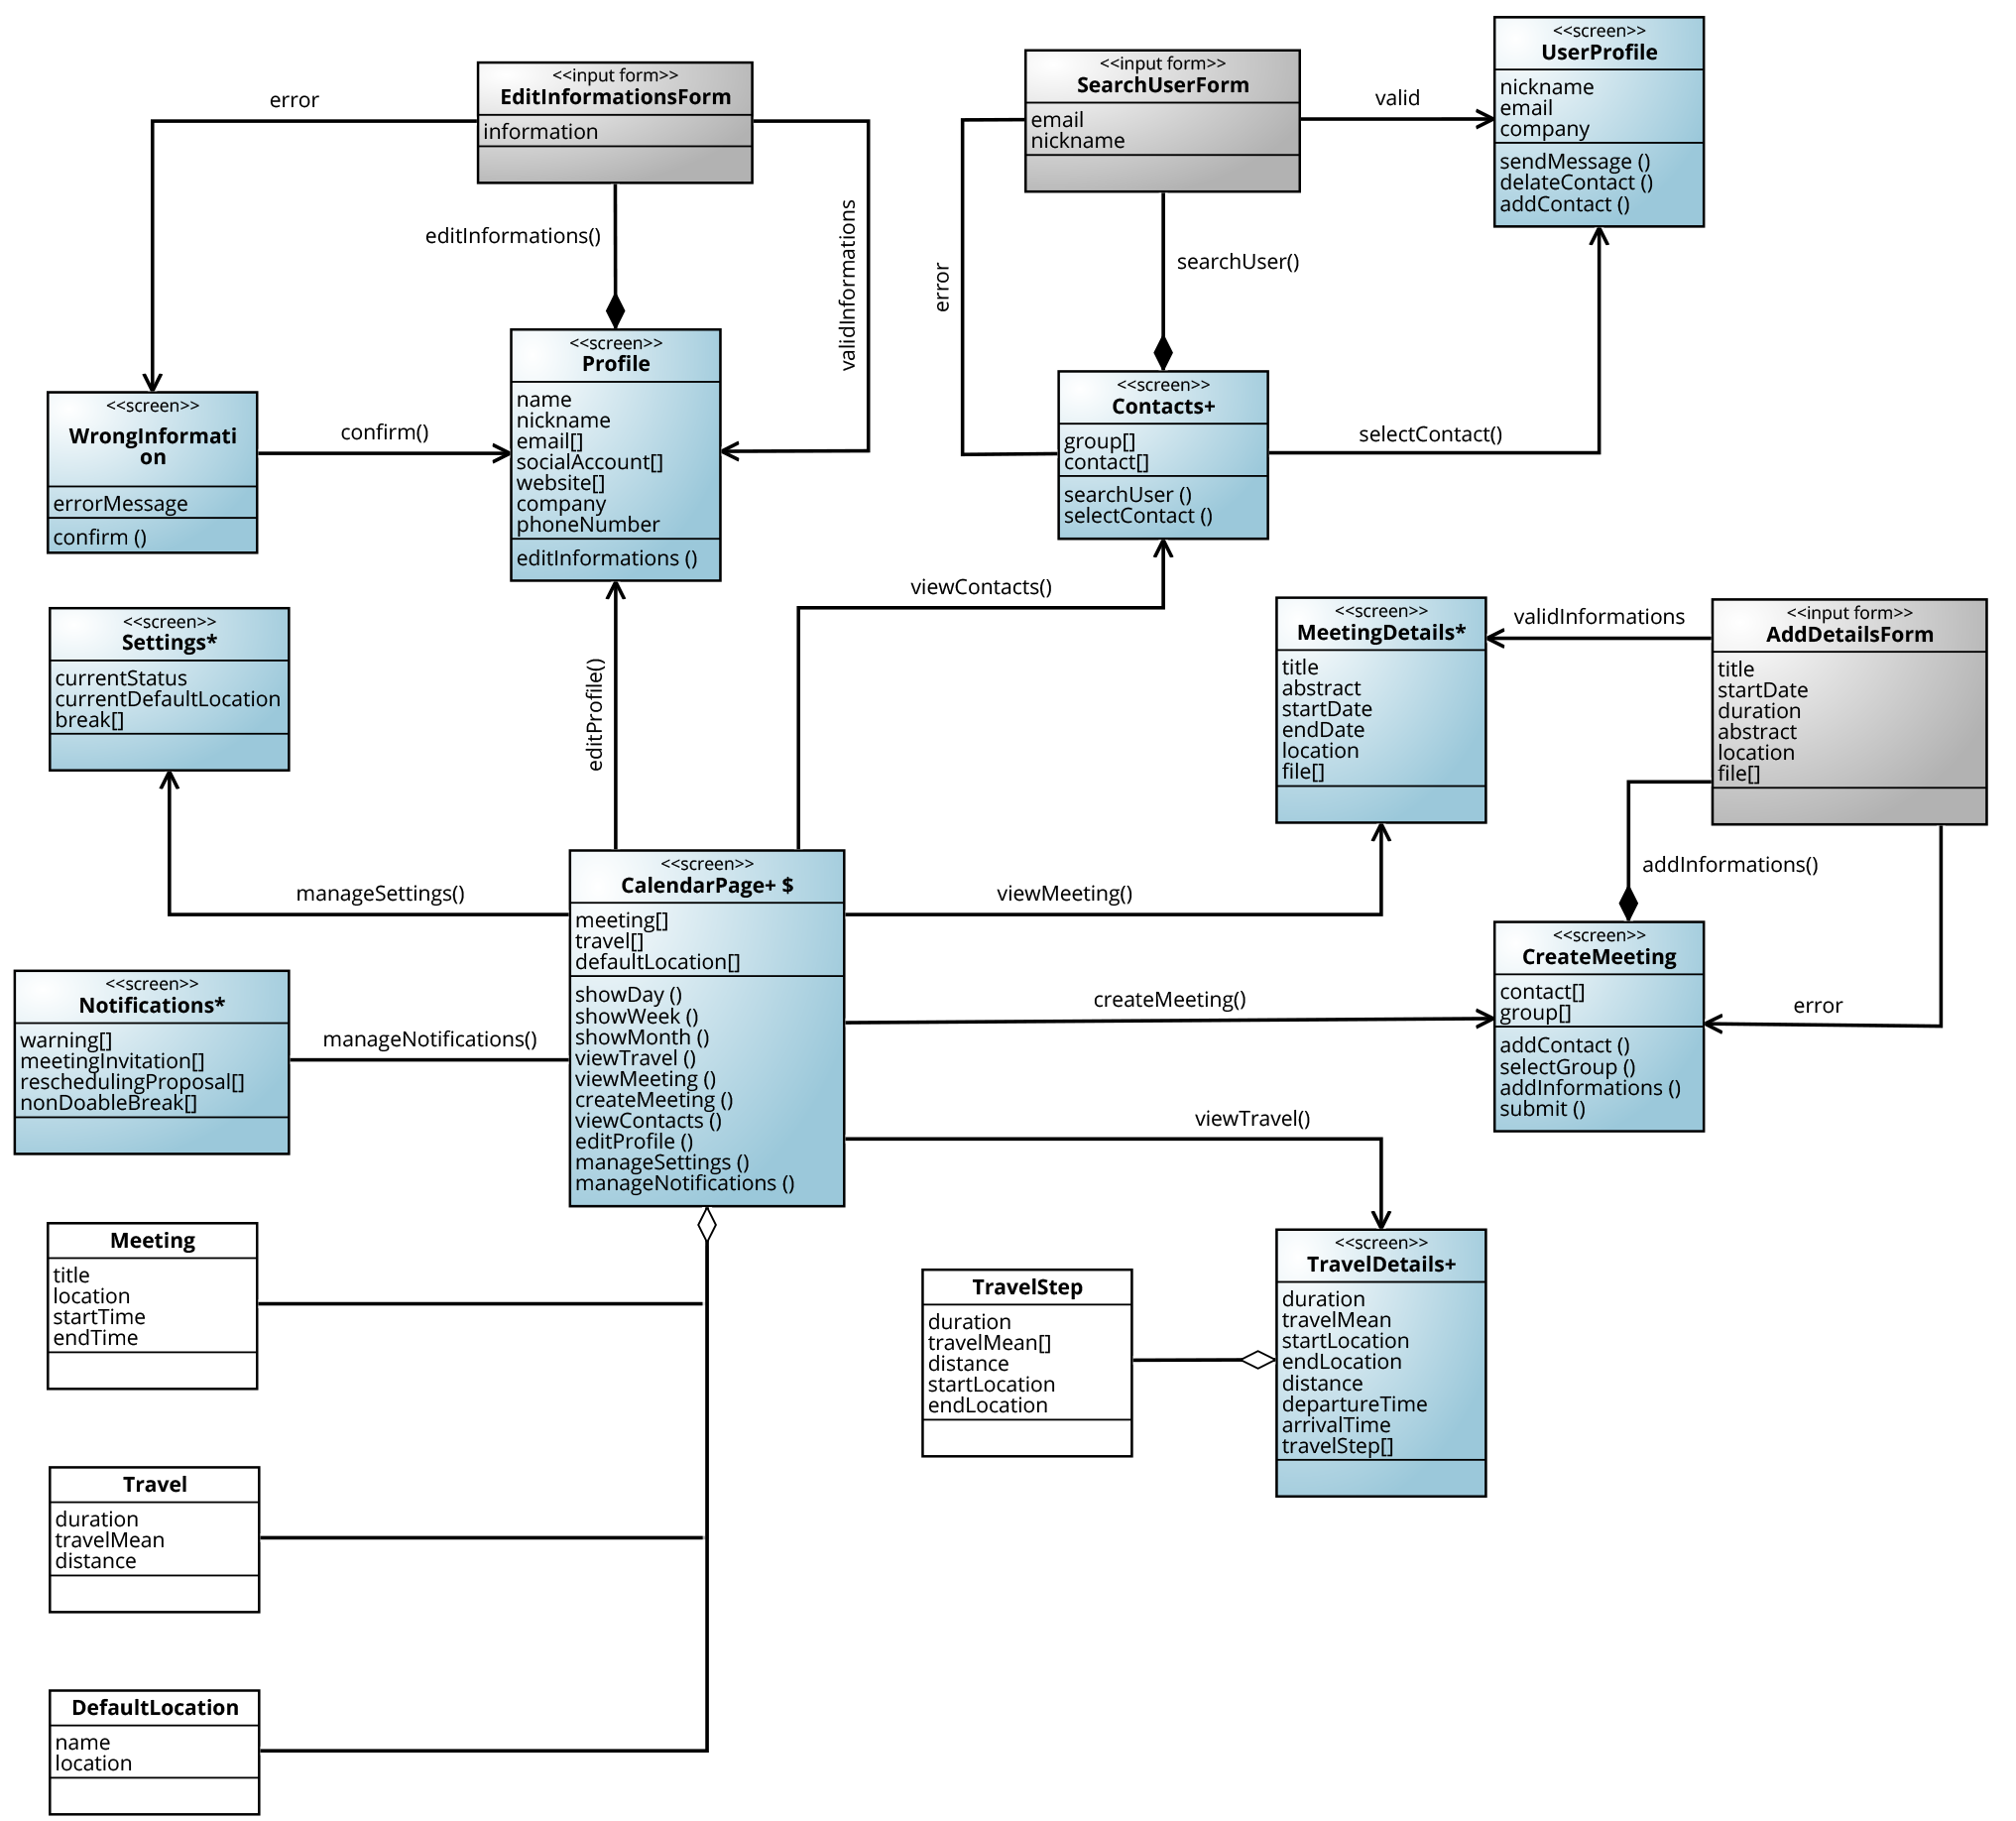
\includegraphics[ width=\textwidth, scale = 1]{Images/UX/UXCalendarPage.png}{}
	\caption{Calendar Page UX}
\end{figure}

\begin{figure}[h]
	\centering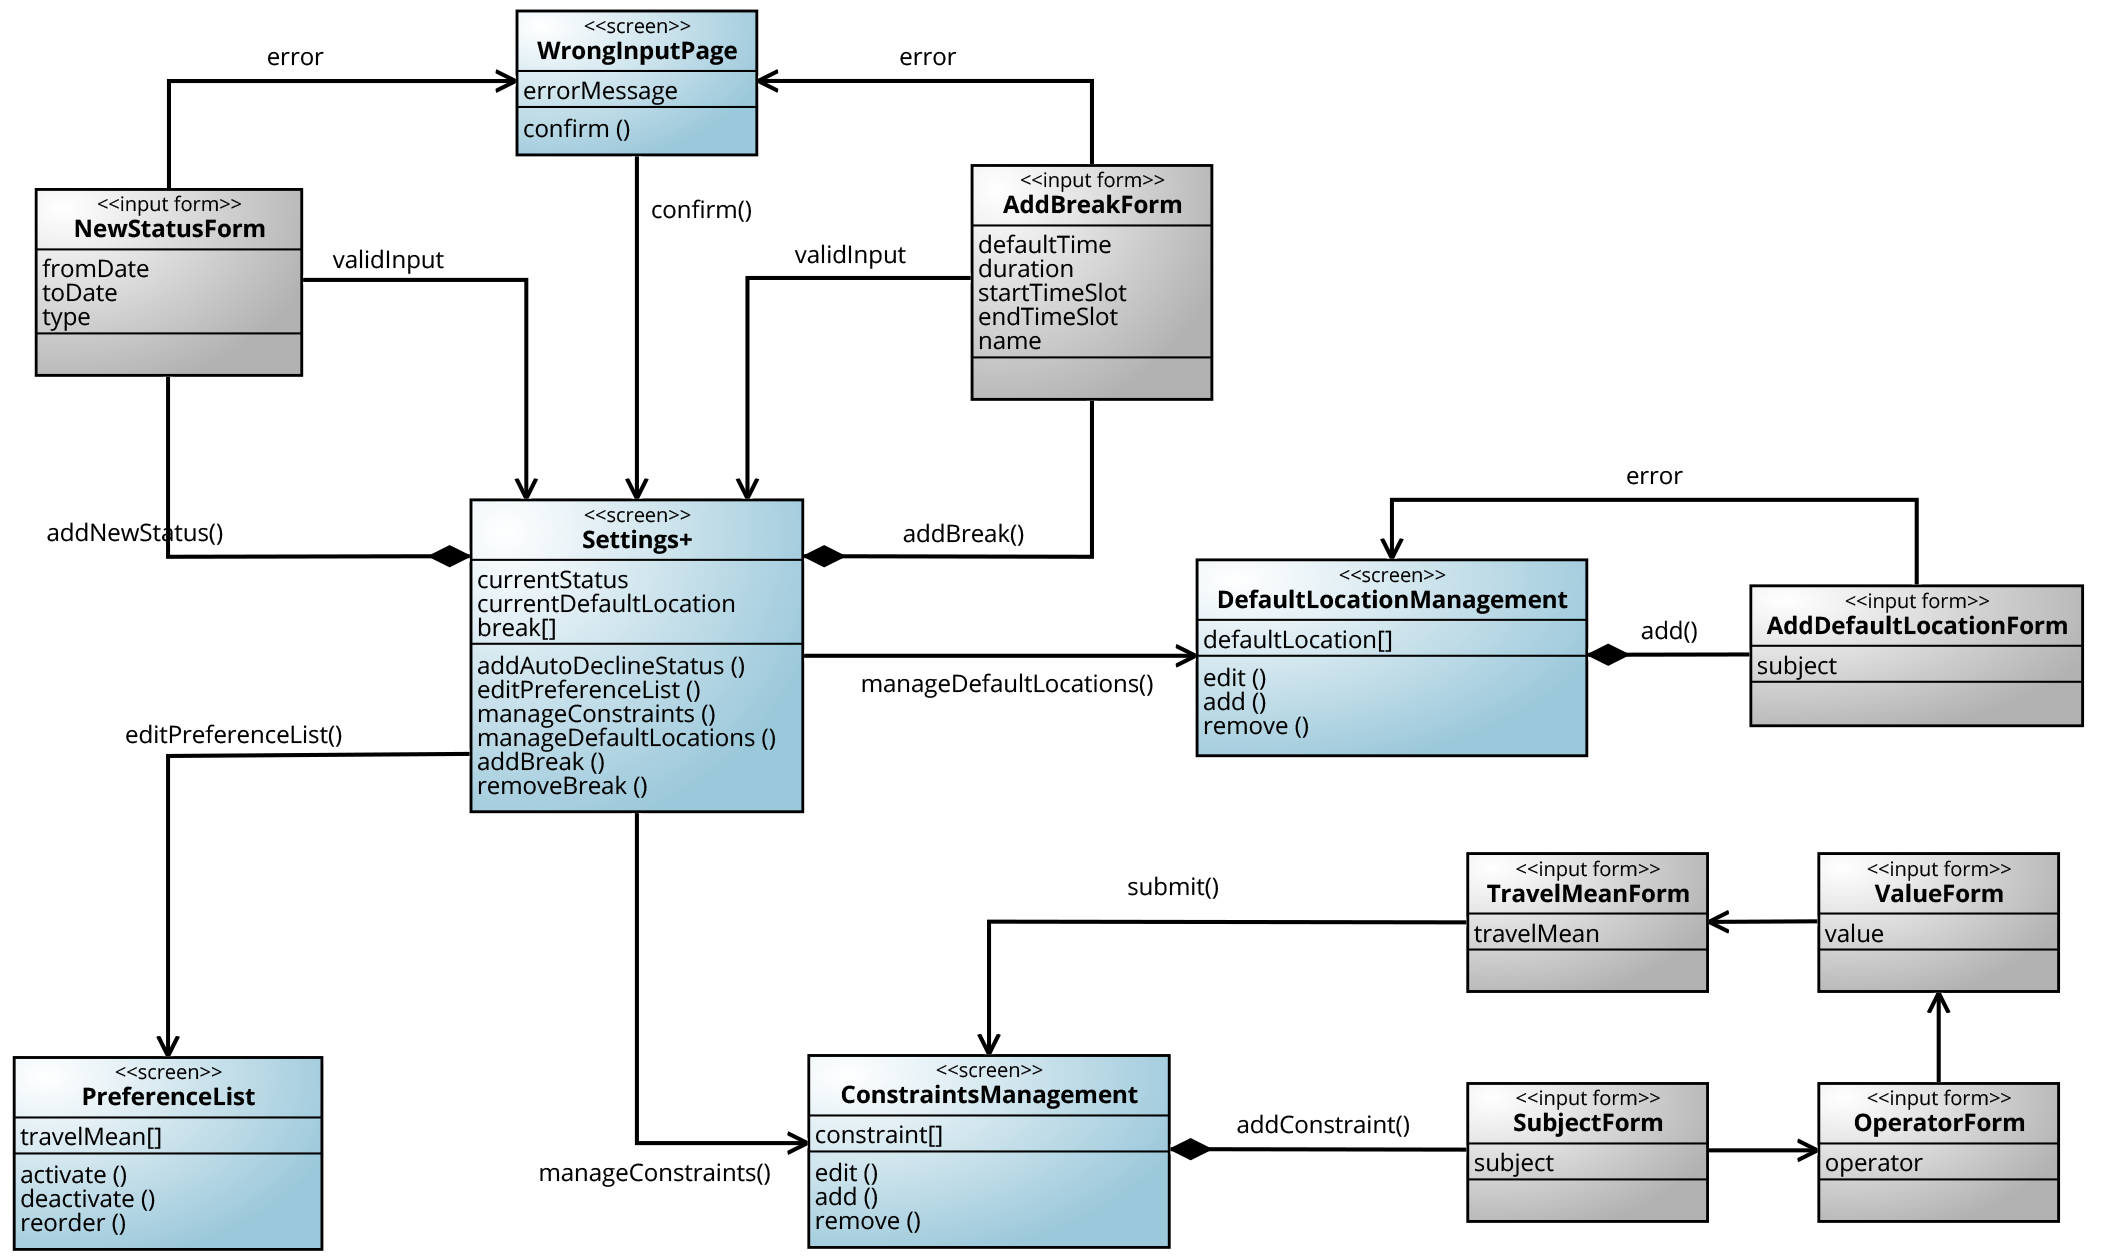
\includegraphics[ width=\textwidth, scale = 1]{Images/UX/UXSettings.png}{}
	\caption{Settings UX}
\end{figure}

\begin{figure}[h]
	\centering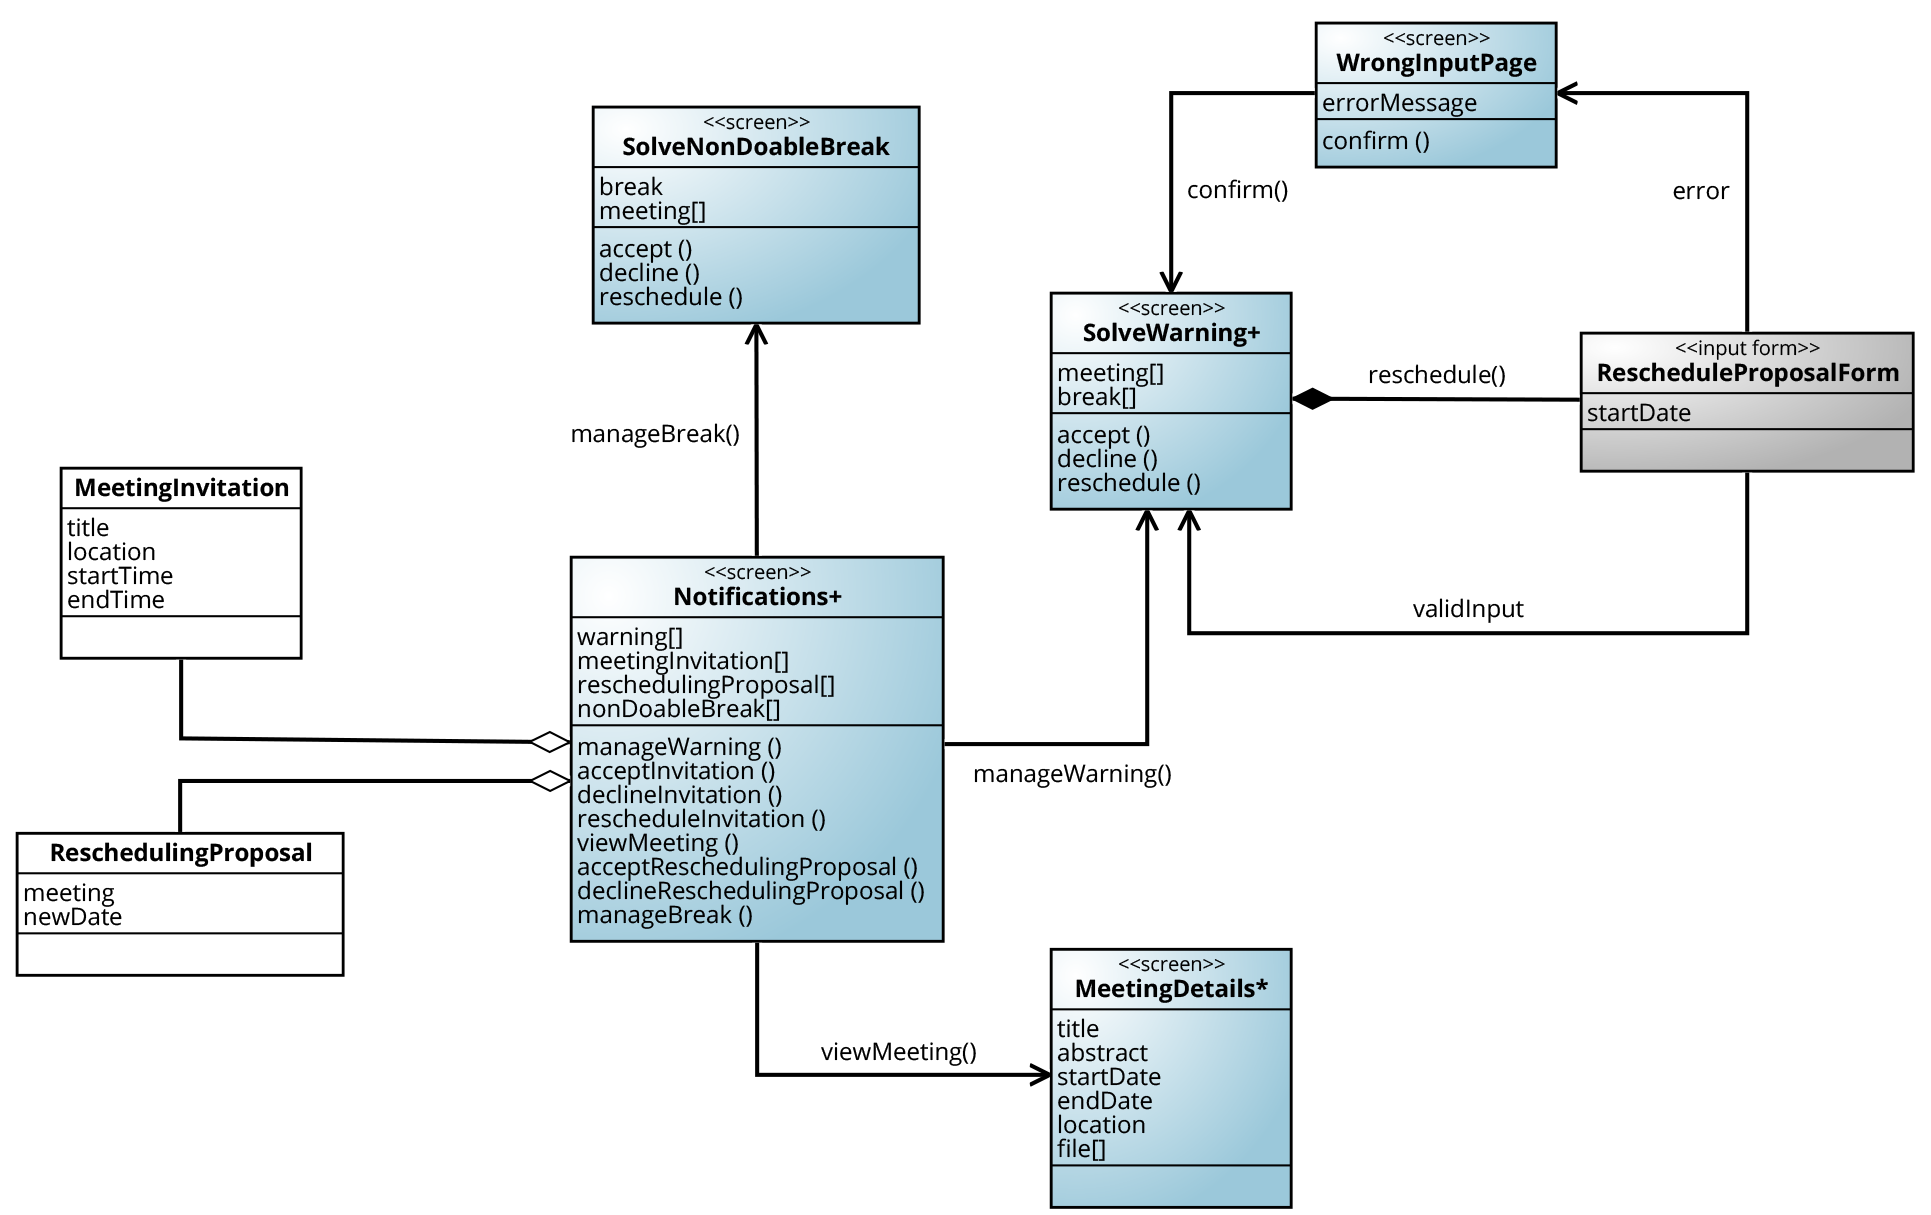
\includegraphics[ width=\textwidth, scale = 1]{Images/UX/UXNotifications.png}{}
	\caption{Notifications UX}
\end{figure}

\begin{figure}[h]
	\centering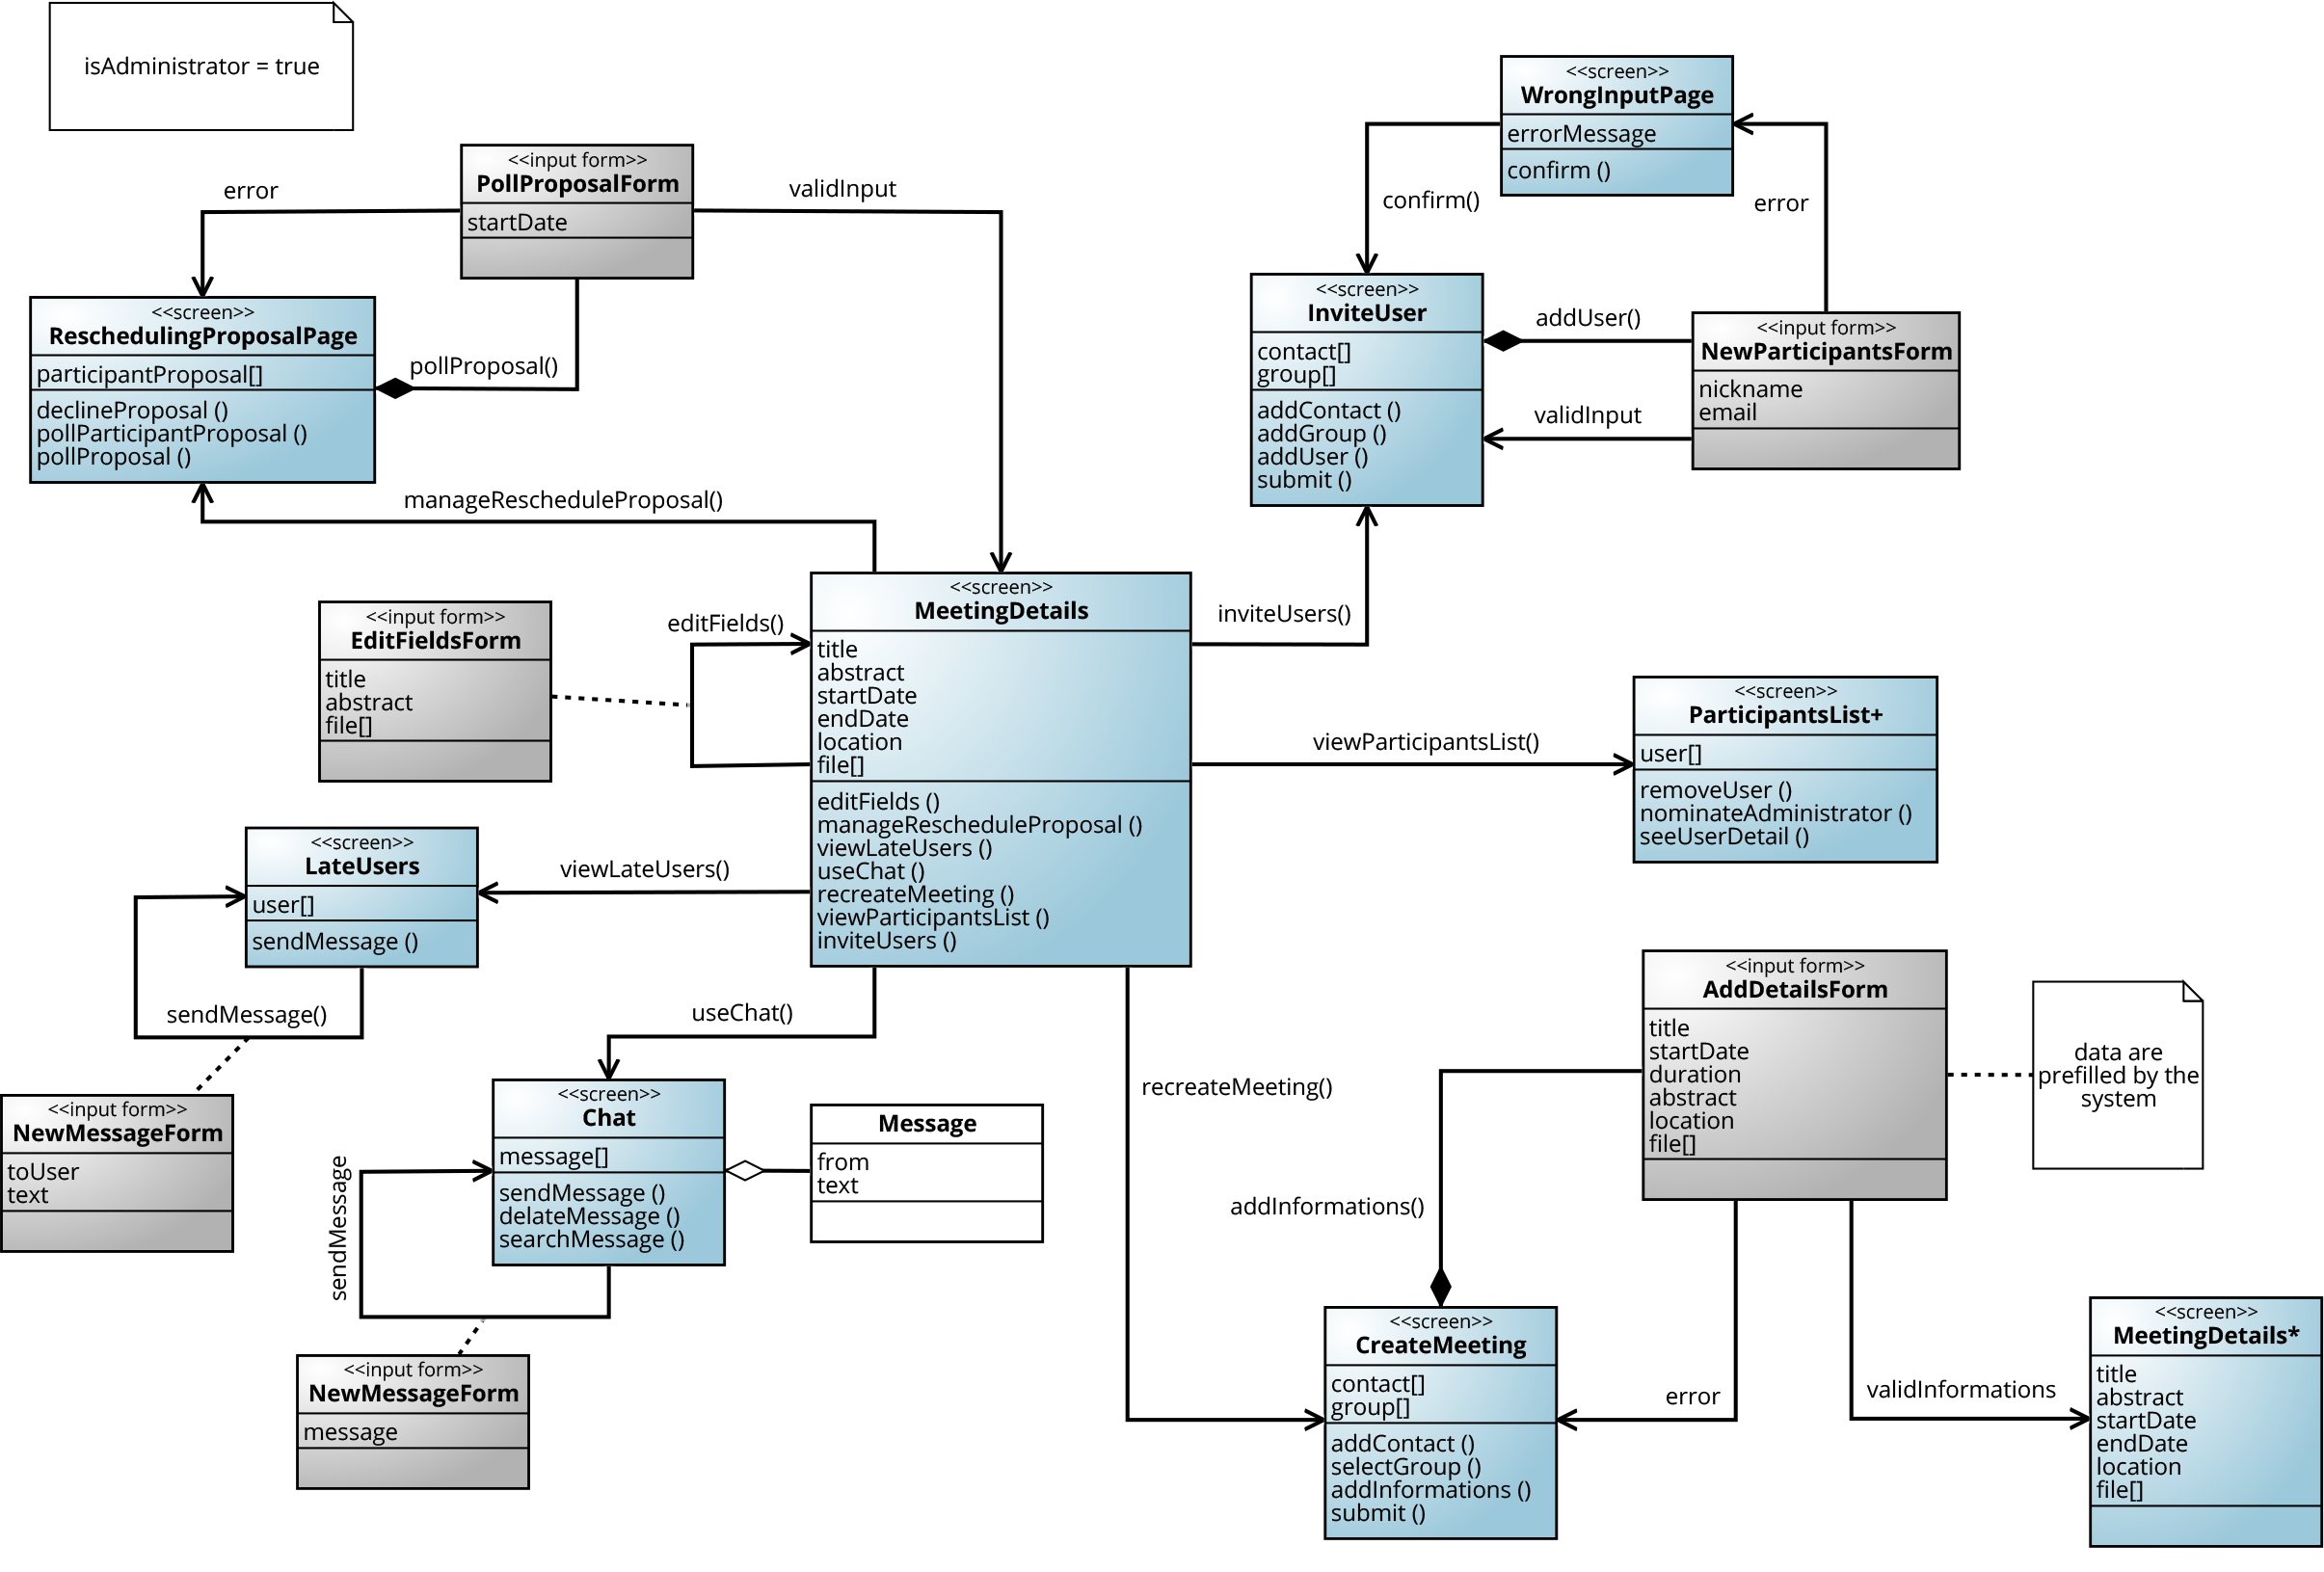
\includegraphics[ width=\textwidth, scale = 1]{Images/UX/UXManageMeeting.png}{}
	\caption{Manage Meeting UX}
\end{figure}
\clearpage